%%% Results %%%
\chapter{Results} \label{ch:results}
In this Section, the methods described are applied to the real data provided and results obtained are presented. As in the previous Section, the segmentation results are divided into segmentation by municipalities and segmentation by way segments of the road network. In addition, the results regarding the map-matching and Poisson regression methods are also included.

\section{Segmentation by municipalities}\label{results:municipalities}
As explained in Section \ref{sec:districts}, the accidents were assigned to the municipality in which they occurred. The relative frequency of accidents was also calculated, which is the number of accidents in that municipality divided by the total number of accidents. In the following table the top 10 municipalities with the most accidents can be seen.
\begin{table}[H]
\centering
\begin{tabular}{|c|c|c|}
\hline
\textbf{Municipality}        & \textbf{Number of accidents} & \textbf{\begin{tabular}[c]{@{}l@{}}Relative\\ frequency\end{tabular}} \\ \hline
Vilniaus miesto savivaldybė  & 2356               & 0.197                                                                 \\ \hline
Kauno miesto savivaldybė     & 1461               & 0.122                                                                 \\ \hline
Klaipėdos miesto savivaldybė & 733                & 0.061                                                                 \\ \hline
Panevėžio miesto savivaldybė & 592                & 0.049                                                                 \\ \hline
Šiaulių miesto savivaldybė   & 468                & 0.039                                                                 \\ \hline
Vilniaus rajono savivaldybė  & 430                & 0.036                                                                 \\ \hline
Kauno rajono savivaldybė     & 347                & 0.029                                                                 \\ \hline
Klaipėdos rajono savivaldybė & 289                & 0.024                                                                 \\ \hline
Panevėžio rajono savivaldybė & 280                & 0.023                                                                 \\ \hline
Šiaulių rajono savivaldybė   & 214                & 0.017                                                                 \\ \hline
\end{tabular}
\captionsetup{justification=centering}
\caption[Accidents by municipality]{Accidents by municipality}
\end{table}
To better visualize these values, they can be plotted over a map using the gmaps Python library \cite{gmaps}. In this case, the relative frequencies were transformed to a colour scale with which the municipality polygons were coloured. 
\begin{figure}[H] 
\centering
\captionsetup{justification=centering}
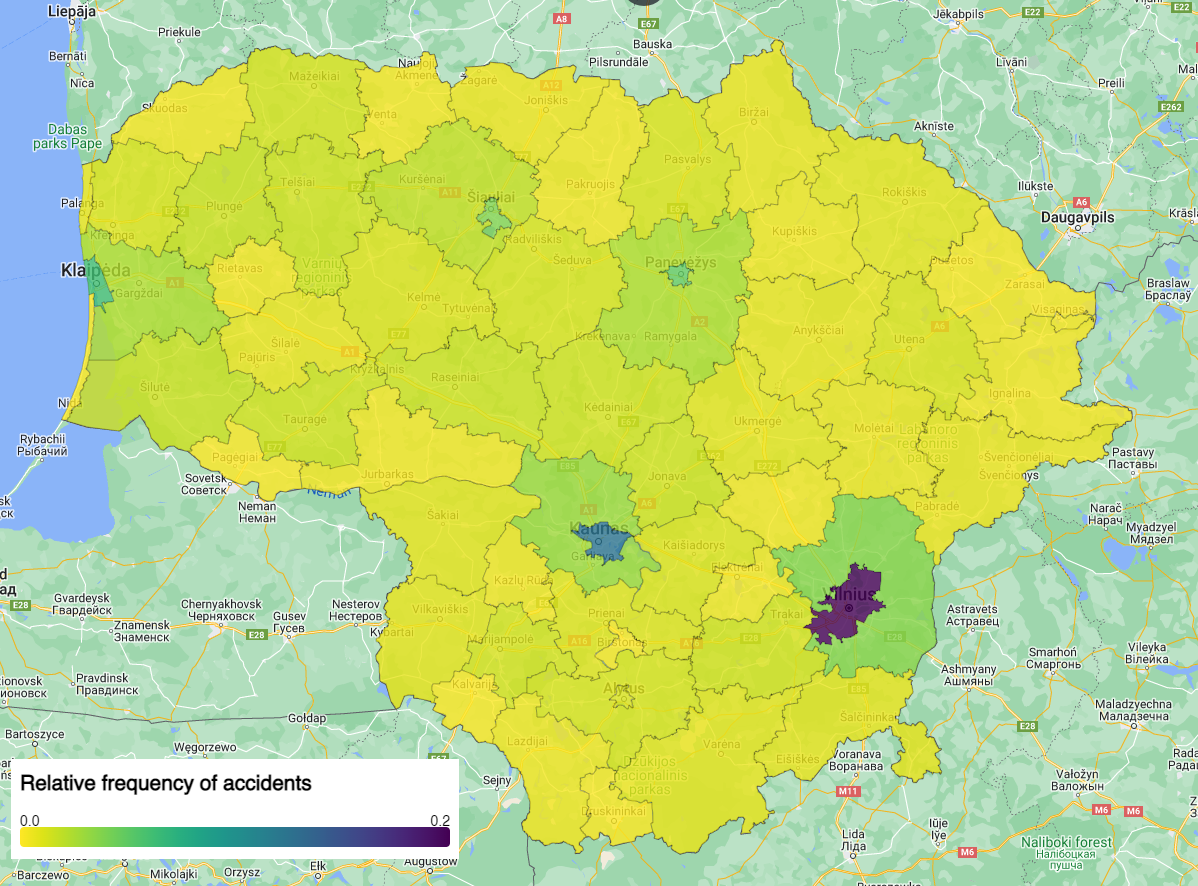
\includegraphics[width=\textwidth]{Images/AccidentsMap.png}
\caption[Relative frequency of accidents by municipality]{Relative frequency of accidents by municipality}
\label{fig:accident_map}
\end{figure}

It can be seen in Figure \ref{fig:accident_map} that the municipalities with the higher intensity of accidents are the ones corresponding to the main populated areas in Lithuania.
According to the Lithuanian municipalitiy's population in January 2022 \cite{population}, the top 10 regions with the most accidents are inside the 20 most populated municipalities. In Table \ref{tab:rank}, the name of the municipality is shown together with its order in the population ranking with Vilniaus in the first row corresponding to the most populated municipality.

\begin{table}[H]
\centering
\begin{tabular}{|c|c|}
\hline
\multicolumn{1}{|c|}{\textbf{\begin{tabular}[c]{@{}c@{}}Municipality ordered\\ by number of accidents\end{tabular}}} & \multicolumn{1}{c|}{\textbf{\begin{tabular}[c]{@{}c@{}}Order in the\\ population ranking\end{tabular}}} \\ \hline
Vilniaus miesto savivaldybė  & 1   \\ \hline
Kauno miesto savivaldybė     & 2  \\ \hline
Klaipėdos miesto savivaldybė & 3 \\ \hline
Panevėžio miesto savivaldybė & 7 \\ \hline
Šiaulių miesto savivaldybė   & 4 \\ \hline
Vilniaus rajono savivaldybė  & 5 \\ \hline
Kauno rajono savivaldybė     & 6 \\ \hline
Klaipėdos rajono savivaldybė & 8 \\ \hline
Panevėžio rajono savivaldybė & 20  \\ \hline
Šiaulių rajono savivaldybė   & 13 \\ \hline
\end{tabular}
\captionsetup{justification=centering}
\caption{Municipalities and their population ranking}
\label{tab:rank}
\end{table}
An additional visualisation has been created where the number of accidents is normalized by the population, showing how likely it is for a person to have an accident when living in each municipality.
\begin{figure}[H] 
\centering
\captionsetup{justification=centering}
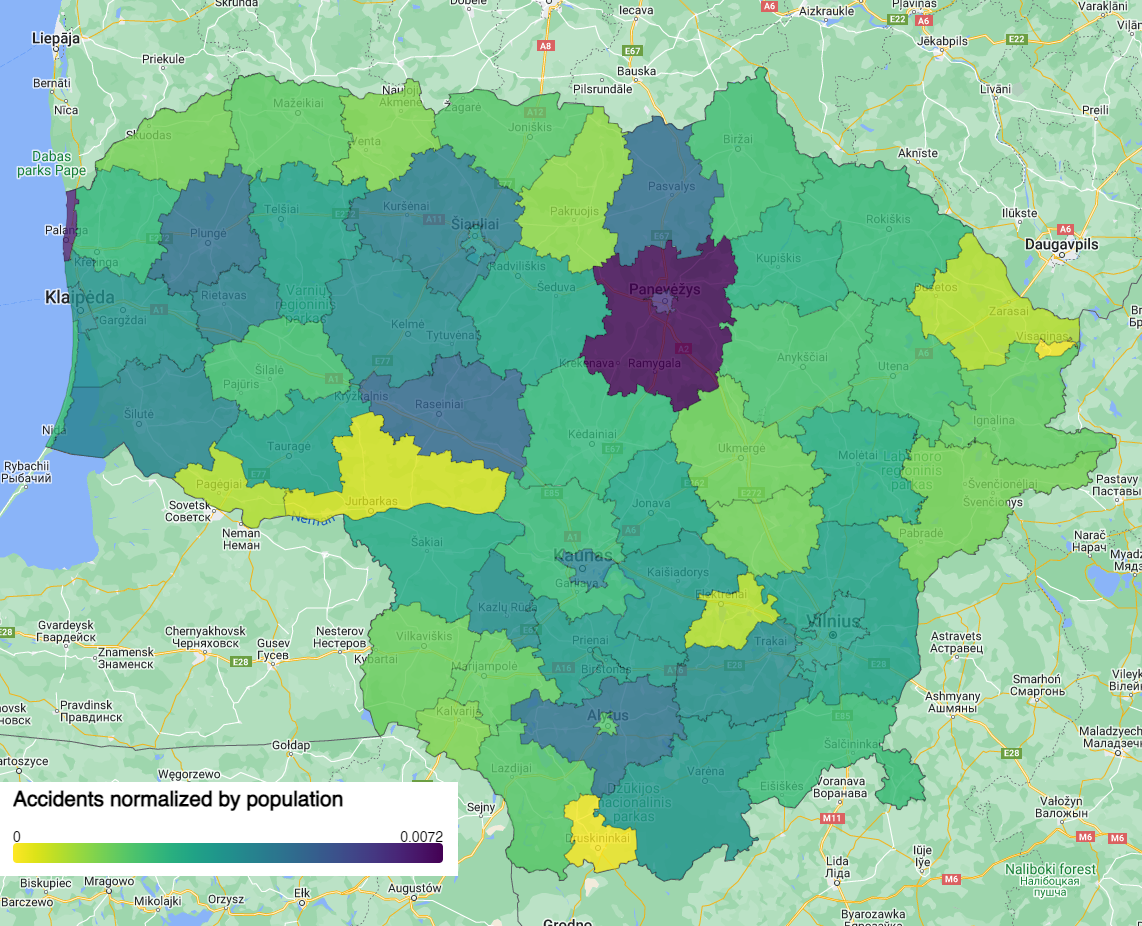
\includegraphics[width=\textwidth]{Images/accpop.png}
\caption[Accidents normalized by population]{Accidents normalized by population}
\label{fig:accident_population}
\end{figure}

\section{Segmentation by way segments}
Initially, the \ac{OSM} \ac{PBF} of Lithuania was read and two DataFrames corresponding to both nodes (Table \ref{tab:nodesdf}) and ways (Table \ref{tab:waysdf}) were created. The steps to create both DataFrames took approximately 2 seconds each.

\begin{table}[H]
\centering
\begin{tabular}{|c|c|c|c|}
\hline
\textbf{nodeId}         & \textbf{latitude} & \textbf{longitude} & \textbf{tags}\\ \hline
15389886                &       54.7309125  &   25.2397012      & [traffic\_signals] \\ \hline
15389895                &       54.7321714  &   25.2436895      & []  \\ \hline
15389899                &       54.7352788  &   25.2467356      & [] \\ \hline
15389959                &       54.7355529  &   25.2458712      & [] \\ \hline
\end{tabular}
\captionsetup{justification=centering}
\caption{Nodes DataFrame}
\label{tab:nodesdf}
\end{table}

\begin{table}[H]
\centering
\begin{tabular}{|c|c|c|}
\hline
\textbf{wayId}         & \textbf{tags }  & \textbf{nodes}\\ \hline
4853620                &       [tertiary, 2, 50, Žvejų g., sign, asphalt] &   [1258016356, 5502503883, ...] \\ \hline
4853621                &       [10, administrative, secondary, 2, yes, 50, ...] &   [31294800, 1754982050, ...] \\ \hline
4853622                &       [residential, 2, Vinco Kudirkos a., asphalt]  &   [31294802, 3647037969, ...] \\ \hline
4853642                &       [secondary, 2, 40, Šventaragio g., ...] &   [31295263, 2778259804, ...]    \\ \hline
\end{tabular}
\captionsetup{justification=centering}
\caption{Ways DataFrame}
\label{tab:waysdf}
\end{table}

To get an idea of the magnitude of this problem, the number of nodes and ways was 21212155 and 137540, respectively. It is worth mentioning that the counting process for such big numbers took around 20 seconds. 
\\
\\
Later, after identifying the intersections as mentioned in the previous Section, the total number of intersections found was 162325. After this step, Algorithm \ref{alg:g0} was applied and it gave the topology graph called $G0$ as a result. The graph structure is formed by vertices specifying the intersection points (including those for the dead end points) and the edges specifying the segments joining them. The edges contain the id of the source and destination edge and their attribute is the way id of the way they belong to, as can be observed in Table \ref{tab:edges_g0}. The vertices consist of the node id and, as an attribute, they incorporate the following information: their latitude and longitude coordinates values and a map that maps each way in which the node appears with the node buffer containing the nodes in that way. The number of vertices and edges were 191991 and 237069, respectively.

\begin{table}[H]
\centering
\begin{tabular}{|c|c|c|}
\hline
\textbf{Source Id}         & \textbf{Destination Id} & \textbf{Edge Attribute: way Id} \\ \hline
32067857                &       56681739 &   137882502 \\ \hline
32070359                &       308851778 &   75265242 \\ \hline
32083634                &       2785419937  &   320804374 \\ \hline
32324789                &       6873079553 &   733863524    \\ \hline
\end{tabular}
\captionsetup{justification=centering}
\caption{Edges of G0}
\label{tab:edges_g0}
\end{table}


\begin{table}[H]
\centering
\begin{tabular}{|c|c|}
\hline
\textbf{Vertex Id}         &  \multicolumn{1}{|c|}{\textbf{\begin{tabular}[c]{@{}c@{}}Vertex Attribute\\ (latitude, longitude, wayMap(wayId -> buffer)\end{tabular}}} \\ \hline
2768460896                &       (54.9056785,23.9441988,Map(271922319 -> ((2768460898,54.9056826,23.9442212), ... )))  \\ \hline
2433869696                &      (54.9433185,23.7571581,Map(235306184 -> ((2433869707,54.9436032,23.7574116), ... )))  \\ \hline
4056430496                &       (55.4694212,22.5209998,Map(403916943 -> ((2339348189,55.4688876,22.5197411), ... )))  \\ \hline
7575735993                &       (54.6453908,25.3811082,Map(277653466 -> ((1258118692,54.6455437,25.3809540), ... )))  \\ \hline
\end{tabular}
\captionsetup{justification=centering}
\caption{Vertices of G0}
\label{tab:vertices_g0}
\end{table}


The second procedure is to add the distance information to $G0$, according to Algorithm \ref{alg:g0distances}. In this case, some information was added to the graph but its structure was not modified. Thus, the number of edges and vertices remained the same. It is shown in Table \ref{tab:edges_g0dist} how the distance information between the source and the destination vertex has been added to the edge attribute. 
\begin{table}[H]
\centering
\begin{tabular}{|c|c|c|}
\hline
\textbf{Source Id}         & \textbf{Destination Id} &   \multicolumn{1}{|c|}{\textbf{\begin{tabular}[c]{@{}c@{}}Edge Attribute\\ (wayId,  distance (source, destination))\end{tabular}}} \\ \hline
32067857                &       56681739 &   (137882502, 455.7275595) \\ \hline
32070359                &       308851778 &  (75265242, 135.1346101) \\ \hline
32083634                &       2785419937  &(320804374, 15.6198426) \\ \hline
32324789                &       6873079553 &(733863524, 212.1690016)    \\ \hline
\end{tabular}
\captionsetup{justification=centering}
\caption{Edges of G0 with distance information}
\label{tab:edges_g0dist}
\end{table}
The last graph transformation is described in Algorithms \ref{alg:g1_1} and \ref{alg:g1_2} and it consists of the segmentation of $G0$ according to a distance threshold. For this procedure the distance obtained before is used. Later, Algorithm \ref{alg:dead_end} is also applied. As expected, the number of both edges and vertices after splitting the previous edges has increased. Now the resulting graph consists of 1469364 edges and 685121 vertices. G1 graph has exactly the same structure regarding edges and vertices as G0 with the distance information (Tables \ref{tab:vertices_g0} and \ref{tab:edges_g0dist}), but in this case the distances have been modified since the edges have been split according to the distance threshold selected (100 meters in this case), and new vertices have been created. 
\\
\\
The computation of each graph was very fast, a few minutes, including the time taken for the count of edges and vertices or even the commands corresponding to show a sample of them. After all of this processing, the result is a graph whose vertices are the \ac{OSM} nodes for Lithuania and whose edges are the segments connecting those vertices. 
\\
\\
To summarize and understand better the process of segmentation of the road network, the number of edges and vertices for each graph is collected in Table \ref{tab:graphs}:
\begin{table}[H]
\centering
\begin{tabular}{|c|c|c|}
\hline
\textbf{Graph}         & \textbf{Number of vertices} & \textbf{Number of edges} \\ \hline
G0                &                      191991 &           237069     \\ \hline
G0 + distances    &                      191991 &           237069 \\ \hline
G1                &                      685121     &      1469364   \\ \hline
\end{tabular}
\captionsetup{justification=centering}
\caption{Number of vertices and edges in each graph}
\label{tab:graphs}
\end{table}

\section{Connected component and PageRank in G0}
After keeping only the largest connected component with 138552 vertices from G0 and applying the PageRank algorithm to the undirected graph, each vertex (intersection) has a score associated with it. This way, after matching each accident with its closest intersection, the value of the intersection's PageRank score is known. Table \ref{tab:pagerank} shows the first five rows corresponding to the intersections with highest PageRank score. Checking them manually, they all correspond to intersections having four incoming/outgoing roads on it.
\begin{table}[H]
\centering
\begin{tabular}{|c|c|}
\hline
\textbf{Intersection Id}         & \textbf{PageRank score}  \\ \hline
309851490                &                      2.3145  \\ \hline
287439601                &                      2.3145  \\ \hline
834526731                &                      2.2535  \\ \hline
8149898695                &                      2.2535  \\ \hline
677323816                &                      2.2487  \\ \hline
\end{tabular}
\captionsetup{justification=centering}
\caption{Top intersections' PageRank score}
\label{tab:pagerank}
\end{table}


\section{GeoMatch: matching accidents with intersections}\label{sec:results_geomatch}
The algorithm described in Section \ref{sec:map_matching} is used now to map the accidents on the road network. To use it in the Poisson regression model, each accident is matched with its nearest intersection in order to associate the PageRank score of that intersection with it. Then, the road network graph that contains the intersection nodes will be selected as the first data set for GeoMatch and the accident points as the second one. GeoMatch is then executed in order to match each accident with its nearest intersection.
\begin{table}[H]
\centering
\begin{tabular}{|c|c|}
\hline
\textbf{Accident id and coordinates}         & \textbf{Intersection matched Id and coordinates}  \\ \hline
LT2019491642, [5204895, 3619151]             &  9241442307, [5204901, 3619145]   \\ \hline
LT2019496092, [5205450, 3621627]   &               2121192109, [5205396, 3621674] \\ \hline
LT2019497006, [5297422, 3612178]            &    32083732, [5297419, 3612173]  \\ \hline
LT2019503187, [5244895, 3564930]             &    986691627, [5245187, 3565017] \\ \hline
\end{tabular}
\captionsetup{justification=centering}
\caption{Accidents and their closest intersection}
\label{tab:acc_inters}
\end{table}

Note that if features of the \ac{OSM} road network other than the PageRank scores are used as predictors in Poisson regression, including type of road, speed limit, etc., then the map-matching should be restricted to the nearest road segment as opposed to the nearest intersection. The methods developed here allow for such experimental designs.


\section{Poisson Regression}\label{sec:results_regression}
Using the information obtained after applying the segmentation and GeoMatch, the distance between each accident and its closest intersection (using the geodesic distance again) was measured with the purpose of using this measure in the log-linear model as a continuous measurement. 

\begin{table}[H]
\centering
\begin{tabular}{|c|c|}
\hline
\textbf{Accident Id}         & \multicolumn{1}{|c|}{\textbf{\begin{tabular}[c]{@{}c@{}}Distance from the accident to\\ the nearest intersection (m)\end{tabular}}}  \\ \hline
LT2019491642               &  8.4683  \\ \hline
LT2019496092             &  71.4226 \\ \hline
LT2019497006            &    5.8211 \\ \hline
LT2019503187              &    305.5852  \\ \hline
\end{tabular}
\captionsetup{justification=centering}
\caption{Distance from accidents to their closest intersection}
\label{tab:acc_inters_dist}
\end{table}

Now that the accidents are matched with their closest intersections, it is easy to put together the accident id with the PageRank score of the corresponding intersection as shown in Table \ref{tab:acc_inters_pagerank}.
\begin{table}[H]
\centering
\begin{tabular}{|c|c|c|}
\hline
\textbf{Accident Id}         & \textbf{Intersection Id} & \textbf{Pagerank score} \\ \hline
LT2019504277               &  1777156623  &  1.2599\\ \hline
LT2019490710             &  2036731935 &  1.7267\\ \hline
LT2017463577            &   2780968063 & 1.0121\\ \hline
LT2019502731              &   455050143 & 0.9968\\ \hline
\end{tabular}
\captionsetup{justification=centering}
\caption{Accidents with their closest intersection's PageRank score}
\label{tab:acc_inters_pagerank}
\end{table}

This information was added to the data previously available from the accident (weather, road conditions, etc.) and the transformations and algorithms described in Section \ref{sec:regresion} were applied. First transforming the disparate discrete values into consecutive values, then encoding them with a One-Hot encoder so they can be processed in a regression and finally grouping all the parameters into a single feature input for the \textit{GeneralizedLinearRegression()} model.
\\
\\
Table \ref{tab:conditions} shows the 12 first rows when grouping the accidents by the same conditions and sorting them in descending order, to visualise which conditions were in place when the most number of accidents happened.  
\begin{table}[H]
\centering
\begin{tabular}{|c|c|c|c|c|c|}
\hline
\textbf{Weather} & \textbf{Light} & \textbf{\begin{tabular}[c]{@{}c@{}}Urban\\ area\end{tabular}} & \textbf{\begin{tabular}[c]{@{}c@{}}Surface\\ condition\end{tabular}} & \textbf{\begin{tabular}[c]{@{}c@{}}Distance to \\ intersection (m)\end{tabular}} & \textbf{\begin{tabular}[c]{@{}c@{}}Number of\\ accidents\end{tabular}} \\ \hline
Clear & Daylight & Yes & Dry & 10 & 661 \\ \hline
Clear & Daylight & Yes & Dry & 0 & 654 \\ \hline
Clear & Daylight & Yes & Dry & 20 & 457 \\ \hline
Clear & Daylight & Yes & Dry & 30 & 401 \\ \hline
Clear & Daylight & Yes & Dry & 40 & 359 \\ \hline
Clear & Daylight & Yes & Dry & 50 & 329 \\ \hline
Clear & Daylight & Yes & Dry & 60 & 259 \\ \hline
Clear & Daylight & Yes & Dry & 70 & 249 \\ \hline
Clear & Daylight & Yes & Dry & 90 & 183 \\ \hline
Clear & Daylight & Yes & Dry & 80 & 172 \\ \hline
Clear & Daylight & Yes & Wet & 10 & 150 \\ \hline
Clear & Daylight & No & Dry & 10 & 122 \\ \hline
\end{tabular}
\captionsetup{justification=centering}
\caption{Top count of accidents with the same conditions}
\label{tab:conditions}
\end{table}

Running this regression model returned a list of features (variables) with their coefficients and standard error together with other statistical measurements from the regression such as the p-value. The coefficient of the feature represents the change in the mean response for one unit of change in that term and the p-value measures the probability of evidence against the null hypothesis (lower probabilities provide stronger evidence). 
%Since the standard error and p-values were low, they do not have much interest for this analysis and were not included in the results.
\\
\\
First, the regression model was run grouping all the data from the 4 years together by the accident conditions and distance to the nearest intersection and counting the number of accidents with those same factors. This result is presented in Table \ref{tab:regression}, where a variable with higher coefficient has higher impact on the number of accidents and one with the lower coefficient has a lower impact on the accident. 
\\
\begin{table}[h]
\centering
\begin{tabular}{|c|c|c|c|c|}
\hline
\textbf{Parameter}       & \textbf{Value}              & \textbf{Coefficient} & \textbf{Std Error} & \textbf{P value} \\ \hline
Light                    & Daylight                    & 1.6264               & 0.0608             & 0.0000           \\ \hline
Surface                  & Dry                         & 1.4060               & 0.0706             & 0.0000           \\ \hline
Weather                  & Clear                       & 1.3470               & 0.0604             & 0.0000           \\ \hline
Weather                  & Rain                        & 0.7179               & 0.0642             & 0.0000           \\ \hline
Urban area               & Yes                         & 0.4765               & 0.0919             & 0.0000           \\ \hline
Light                    & Darkness, street lights lit & 0.2596               & 0.0631             & 0.0000           \\ \hline
Distance to intersection & -                           & -0.0055              & 0.0001             & 0.0000           \\ \hline
Weather                  & Hail                        & -0.2006              & 0.0735             & 0.0063           \\ \hline
Light                    & Darkness, no street lights  & -0.2603              & 0.0645             & 0.0001           \\ \hline
Surface conditions       & Slippery                    & -0.8660              & 0.0979             & 0.0000           \\ \hline
\end{tabular}
\captionsetup{justification=centering}
\caption{Poisson Regression - Influence of parameters on the accident count}
\label{tab:regression}
\end{table}

Then, several more regressions were run grouping the data differently, including more or less features or even doing regressions with individual features. The results were consistent and similar, for example the case presented in Table \ref{tab:regression2} is done by grouping the accidents by month. %and year.
\\
\begin{table}[h]
\centering
\begin{tabular}{|c|c|c|c|c|}
\hline
\textbf{Parameter}       & \textbf{Value}             & \textbf{Coefficient} & \textbf{Std Error} & \textbf{P value} \\ \hline
Light                    & Daylight                   & 0.5623               & 0.0612             & 0.0000           \\ \hline
Surface                  & Dry                        & 0.4056               & 0.0742             & 0.0000           \\ \hline
Urban area               & Yes                        & 0.2765               & 0.0920             & 0.0027           \\ \hline
Weather                  & Clear                      & 0.1716               & 0.0626             & 0.0061           \\ \hline
Weather                  & Rain                       & 0.0457               & 0.0659             & 0.4878           \\ \hline
Distance to intersection & -                          & -0.0012              & 0.0001             & 0.0000           \\ \hline
Weather                  & Hail                       & -0.0064              & 0.0863             & 0.9403           \\ \hline
Light                    & Darkness, no street lights & -0.0243              & 0.0651             & 0.7087           \\ \hline
Surface conditions       & Slippery                   & -0.0997              & 0.1172             & 0.3947           \\ \hline
\end{tabular}
\captionsetup{justification=centering}
\caption{Poisson Regression - Influence of parameters on the accident count by month}
\label{tab:regression2}
\end{table}

If a coefficient is positive it means that it affects the mean number of accidents when it increases and vice versa. Since most parameters are categorical in this case and, after the transformations, can only take values 0 or 1, how much they affect the count is limited. The continuous parameters in this analysis are the distance to the intersection that is close to 0 and the PageRank score of that intersection that is a high negative.
\\
\\
The equation that models the parameter $\lambda$, the mean number of accidents in a month given the results in Table \ref{tab:regression2} would be:
\begin{align}
    log(\lambda) = 0.0989 &+ 0.5623\:daylight + 0.4056\:dry + 0.2765\:urban + 0.1716\:clear \\ + 0.0457\:rain & - 0.0012\:distance - 0.0064\:hail - 0.0243\:no\_lights - 0.0997\:slippery \nonumber
\end{align}
with 0.0989 being the intercept resulting from the Poisson regression. 
\\
\\
For example, the \textit{"Light: Daylight"} condition value would increase the mean by a factor of $e^{0.5623}=1.75$ or increases it by 75\%, and the \textit{"Weather: Hail"} would decrease the mean by a factor of $e^{-0.0064}=0.9936$ or decreases it by 0.64\%.
\\
\\
When grouping the counts of accidents to perform the previous  Poisson regressions, the PageRank score is not used because there is not enough data to differentiate different factors even upon discretizing the PageRank scores. Therefore, a separate analysis was done using only the PageRank score of the accident's closest intersection and the result was -0.5405 as its coefficient, meaning that a high PageRank score decreases the number of accidents. This seems to indicate that, without considering the distance to the nearest intersection, the number of accidents seems to decrease as the PageRank score of the nearest intersection increases.
\\
\\
A last Poisson regression model was done considering the distance to nearest intersection together with the PageRank score and using them as the predictors. The result obtained in this case is consistent with the previous ones, getting -0.0050 and -0.5778 as the coefficients for the distance and PageRank score, respectively. Their interpretation is the same mentioned before, they both decrease the number of accidents as their values increase. 

\begin{comment}
\\
\begin{table}[h]
\centering
\begin{tabular}{|c|c|c|}
\hline
\textbf{Parameter}         & \textbf{Value}  & \textbf{Coefficient} \\ \hline
Closest intersection PageRank score &    - & -0.2376 \\ \hline
\end{tabular}
\captionsetup{justification=centering}
\caption{Poisson Regression - Influence of PageRank score}
\label{tab:regression}
\end{table}
\end{comment}

